\section{Scheduler}

\subsection{Question - Priority Feedback Queue}

\vspace{0.5cm}

\textbf{QUESTION}: What is the advantage of using priority feedback queue in comparison with other scheduling algorithms you have learned?

\vspace{0.5cm}

Giải thuật Priority Feedback Queue (PFQ) sử dụng tư tưởng của một số giải thuật khác gồm giaỉ thuật Priority Scheduling - mỗi process mang một độ ưu tiên để thực thi, giải thuật Multilevel Queue - sử dụng nhiều mức hàng đợi các process, giải thuật Round Robin - sử dụng quantum time cho các process thực thi. Dưới đây là các giải thuật định thời khác đã học:

\vspace{0.5cm}

\begin{itemize}
	\item First Come First Served (FCFS)
	\item Shortest Job First (SJF)
	\item Shortest Remaining Time First (SRTF)
	\item Priority Scheduling (PS)
	\item Round Robin (RR)
	\item Multilevel Queue Scheduling (MLQS)
	\item Multilevel Feedback Queue (MLFQ)
\end{itemize}

\vspace{0.5cm}

Cụ thể, giải thuật PFQ sử dụng 2 hàng đợi là $ ready\_queue $ và $ run\_queue $ với ý nghĩa như sau:

\vspace{0.5cm}

\begin{itemize}
	\item $ ready\_queue $: hàng đợi chứa các process ở mức độ ưu tiên thực thi trước hơn so với hàng đợi $ run\_queue $. Khi CPU chuyển sang slot tiếp theo, nó sẽ tìm kiếm process trong hàng đợi này. 
	\item $ run\_queue $: hàng đợi này chứa các process đang chờ để tiếp tục thực thi sau khi hết slot của nó mà chưa hoàn tất quá trình của mình. Các process ở hàng đợi này chỉ được tiếp tục slot tiếp theo khi $ ready\_queue $ rỗi và được đưa sang hàng đợi  $ ready\_queue $ để xét slot tiếp theo.
	\item Cả hai hàng đợi đều là hàng đợi có độ ưu tiên, mức độ ưu tiên dựa trên mức độ ưu tiên của process trong hàng đợi.
\end{itemize}

\vspace{0.5cm}

\textbf{Ưu điểm của giải thuật PFQ}

\vspace{0.5cm}

\begin{itemize}
	\item Sử dụng time slot, mang tư tưởng của giải thuật RR với 1 khoảng quantum time, tạo sự công bằng về thời gian thực thi giữa các process, tránh tình trạng chiếm CPU sử dụng, trì hoãn vô hạn định.
	\item Sử dụng hai hàng đợi, mang tư tưởng của giải thuật MLQS và MLFQ, trong đó hai hàng đợi được chuyển qua lại các process đến khi process được hoàn tất, tăng thời gian đáp ứng cho các process (các process có độ ưu tiên thấp đến sau vẫn có thể được thực thi trước các process có độ ưu tiên cao hơn sau khi đã xong slot của mình).
	\item Tính công bằng giữa các process là được đảm bảo, chỉ phụ thuộc vào độ ưu tiên có sẵn của các process. Cụ thể xét trong khoảng thời gian $ t0 $ nào đó, nếu các process đang thực thi thì hoàn toàn phụ thuộc vào độ ưu tiên của chúng. Nếu có 1 process $ p0 $ khác đến, giả sử $ ready\_queue $ đang sẵn sàng, process $ p0 $ này vào hàng đợi ưu tiên và phụ thuộc vào độ ưu tiên của nó, cho dù trước đó các process khác có độ ưu tiên cao hơn đã thực thi xong, chúng cũng không thể tranh chấp với process $ p0 $ được vì chúng đang chờ trong  $ run\_queue $ cho đến khi $ ready\_queue $ là rỗi, tức $ p0 $ đã được thực thi slot của nó.
\end{itemize}

\vspace{0.5cm}

\subsection{Result - Gantt Diagrams}
\vspace{0.5cm}
\textbf{REQUIREMENT}: Draw Gantt diagram describing how processes are executed by the CPU.

\vspace{0.5cm}

\textbf{Test 0:}

\vspace{0.5cm}

\begin{figure}[tph]
	\centering
	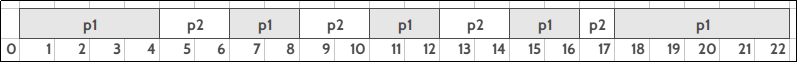
\includegraphics[width=13cm]{Images/sched0.png}
	\vspace{0.5cm}
	\caption{Lược đồ Gantt CPU thực thi các processes - test 0}
	\label{fig:schedtest0}
\end{figure}


\vspace{0.5cm}

Trong test này, CPU xử lí trên 2 process p1 và p2 trong 22 time slot như lược đồ Gantt ở trên.


\vspace{0.5cm}

\textbf{Test 1:}

\vspace{0.5cm}

\begin{figure}[tph]
	\centering
	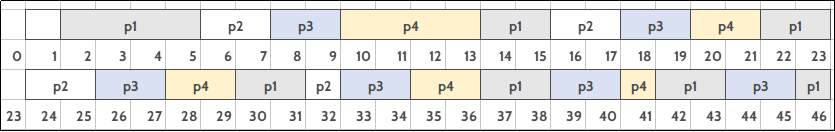
\includegraphics[width=15cm]{Images/sched1.png}
	\vspace{0.5cm}
	\caption{Lược đồ Gantt CPU thực thi các processes - test 1}
	\label{fig:schedtest1}
\end{figure}

\vspace{0.5cm}

Trong test này, CPU xử lí trên 4 process p1, p2, p3 và p4 trong 46 time slot như lược đồ Gantt ở trên.


\vspace{0.5cm}

\subsection{Implementation}
\subsubsection{Priority Queue}

Hàng đợi ưu tiên trong trường hợp này xử lý cho không quá 10 process, do đó, ta đơn giản chỉ cần dùng vòng lặp để xử lý chức năng mà một hàng đợi ưu tiên cần có.

Cụ thể với hàm  $ enqueue() $, ta chỉ cần đưa vào cuối hàng đợi nếu sẵn sàng (còn trống). Với hàm $ dequeue() $, ta duyệt tìm process có độ ưu tiên cao nhất ra, đồng thời cập nhật lại trạng thái của queue khi xóa 1 phần tử.

Dưới đây là phần hiện thực hàng đợi ưu tiên cho Scheduler.

\lstinputlisting{files/queue.c}


\subsubsection{Scheduler}

Nhiệm vụ của scheduler là quản lý việc cập nhật các process sẽ được thực thi cho CPU. Cụ thể scheduler sẽ quản lý 2 hàng đợi ready và run như ở trên đã mô tả. Trong assignment này, ta chỉ cần hiện thực tiếp hàm tìm một process cho CPU thực thi.

Cụ thể, với hàm o$ get\_proc() $, trả về một process trong hàng đợi ready, nếu hàng đợi ready rỗi, ta cấp nhật lại hàng đợi bằng các process đang chờ cho các slot tiếp theo trong hàng đợi run. Ngược lại, ta tìm ra process có độ ưu tiên cao từ hàng đợi này.

Dưới đây là phần hiện thực của chức năng nói trên.

\lstinputlisting{files/sched.c}